%-------------------------------
\section{Produktdaten}
\label{sec:Produktdaten}
%-------------------------------

\begin{quote}
\begin{tabular}{p{1.5cm}p{14.5cm}}


	 /D10/	& \textbf{Datentyp:} Räume \\
				& \textbf{Attribute:} Raum ID \textsl{(systemintern)}, Raumnummer, Gebäude, Stockwerk, Sitzplätze, PC-Plätze, Beamer, Visualizer, Overheads, Tafeln, Whiteboards  \\[0.25cm]

\end{tabular}


\begin{tabular}{p{1.5cm}p{14.5cm}}
		
	 /D20/	& \textbf{Datentyp:} Lehrstühle \\
				& \textbf{Attribute:} Lehrstuhl ID \textsl{(systemintern)}, Lehrstuhlname, Lehrstuhlinhaber, Fakultät, (Haupt-)Gebäude, (Haupt-)Stockwerk  \\[0.25cm]

\end{tabular}


\begin{tabular}{p{1.5cm}p{14.5cm}}
					
	 /D30/	& \textbf{Datentyp:} Benutzer \\
				& \textbf{Attribute:} Benutzer ID \textsl{(systemintern)}, Benutzerkennung, Passwort (Hash), Salt, E-Mail, Benutzerzugehörigkeit (Verwaltung, betreffender Lehrstuhl, wünschenswerterweise auch Student), Vorname, Nachname, letzter Login  \\[0.25cm]

\end{tabular}


\begin{tabular}{p{1.5cm}p{14.5cm}}
	
	 /D50/	& \textbf{Datentyp:} Lehrveranstaltungen \\
				& \textbf{Attribute:} Veranstaltungs ID \textsl{(systemintern)}, Benutzer ID (Dozent), Veranstaltungskurzbezeichnung, Veranstaltungsname, Semester, Benötigte SWS, Art (Vorlesung|Übung|Tutorium), Freigabe durch Dozent, Beschreibung (Tag, Zeiteinheiten, etc. wird über "Raumbelegung (/D60/)" ermittelt, wo für jede Zeiteinheit ein Eintrag erstellt wird und Veranstaltungen mehrere Einträge pro Semester buchen können.) \\[0.25cm]

\end{tabular}


\begin{tabular}{p{1.5cm}p{14.5cm}}
					
	 /D60/	& \textbf{Datentyp:} Raumbelegungen (aller Freigabestatus-Arten) \\
				& \textbf{Attribute:} Belegungs ID \textsl{(systemintern)}, Veranstaltungs ID (Lehrveranstaltung), Raum ID, Semester, Tag, Zeiteinheit, Freigabestatus (unbearbeite|freigegeben|abgelehtn|gegenvorschlag), Freigabenachricht (Falls ein Vorschlag abgelehnt wurde und dies nun ein reservierter Vorschlag des Status "gegenvorschlag" ist), Kommentar  \\[0.25cm]

\end{tabular}


\begin{tabular}{p{1.5cm}p{14.5cm}}
		
	 /DW70/& \textbf{Datentyp:} Studentenbelegungen \\
				& \textbf{Attribute:} Studenten-Belegungs ID \textsl{(systemintern)}, Benutzer ID (Student), Belegungs ID (freigegebene Lehrveranstaltung) \\[0.25cm]

\end{tabular}


\begin{tabular}{p{1.5cm}p{14.5cm}}
					
	 /DW80/& \textbf{Datentyp:} Ticker-Nachricht \\
				& \textbf{Attribute:} Meldungs ID \textsl{(systemintern)}, Meldungstext, Start-Datum, End-Datum, exklusiv für Lehrstuhl ID ('null' wenn für alle), exklusiv für Veranstaltungs ID ('null' wenn für alle), exklusiv für Raum ID ('null' wenn für alle) \\[0.25cm]
		
\end{tabular}


In Structured-Entity-Relationship-Modell (SERM) wird der Zusammenhang der oben spezifizierten persistent zu speichernden Daten verdeutlicht. \\

\begin{figure}
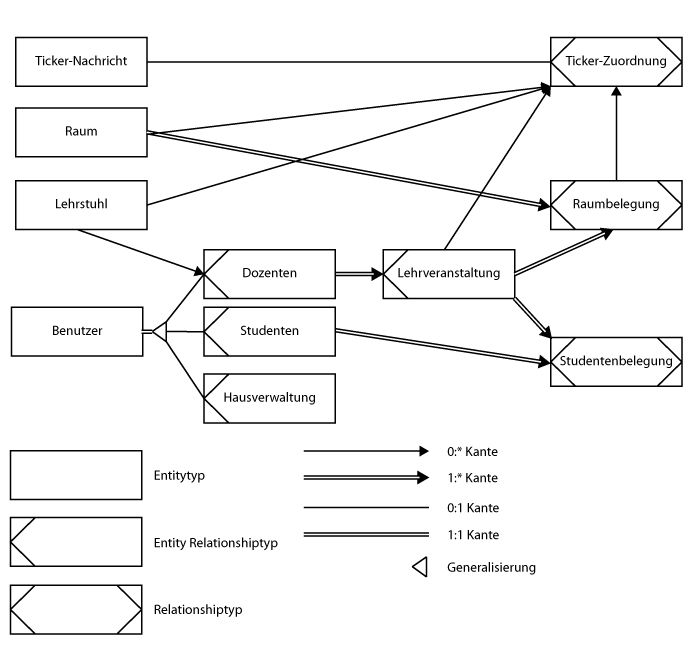
\includegraphics[width=13cm, height=14cm]{./images/section_5/dbserm}
\caption{SERM der Daten-Architektur}
\label{fig:dbserm}
\end{figure}

Wie zu sehen ist, existieren sowohl Räume als auch Lehrstühle als eigenständige Einheiten (Entity). Benutzer können einem Lehrstuhl zugeordnet werden, womit sie der Klasse "Dozent" entsprechen. Sie können aber auch der Klasse "Verwaltung" oder "Student" angehören und somit keinem Lehrstuhl zugeordnet werden. Lehrveranstaltungen müssen einem Benutzer zugeordnet werden, der (allein an der Grafik nicht erkennbar) ein der Klasse "Dozent" angehören muss. Eine Raumbelegung ist keine Einheit sondern eine Zuordnung (Relationship) und muss einer Lehrveranstaltung und einem Raum zugeordnet werden können. Die Zuordnung Studentenbelegung muss einem Benutzer (der Klasse "Student") und einer Raumbelegung zugeordnet werden können. Ticker-Nachrichten können einem Raum, einer Lehrveranstaltung oder einem Lehrstuhl zugeordnet werden, nichts davon ist aber zwingend. \\


\end{quote}